\section{Threshold selection}
\label{sec:thresholding}

With class probabilities a decision can be tuned after the fact: predict the positive class when
$\mu_x(\{\text{positive}\}) \ge t$. We compare the default $t$, the analytic cost threshold
$C_{\text{FP}}/(C_{\text{FP}} + C_{\text{FN}})$, which is optimal under
calibration~\citep{elkan2001cost}, and the threshold that minimizes mean decision cost on
validation examples. German Credit has a canonical cost matrix (\CostRatioGerman); for Breast
Cancer Wisconsin we assume \CostRatioWdbc{} for a missed malignant case and for SST-2 symmetric
costs.

\begin{table}[t]
  \caption{Mean decision cost at the default and the analytic threshold, the validation-selected
    threshold $t$ with its cost, and accuracy before and after selection. Tabular values are
    means over \NRepeats{} split repeats. All models and all metrics are in
    Table~\ref{tab:thresholds-all}, and further sweeps in Figure~\ref{fig:threshold-more}.}
  \label{tab:thresholds}
  \centering\small
  \begin{tabular}{llcccccc}
\toprule
 & & \multicolumn{2}{c}{Cost at fixed $t$} & \multicolumn{2}{c}{Validation-selected} & \multicolumn{2}{c}{Accuracy} \\
\cmidrule(lr){3-4}\cmidrule(lr){5-6}\cmidrule(lr){7-8}
Dataset & Model & default & analytic & $t$ & cost & default & selected \\
\midrule
\multirow{2}{*}{German Credit} & Jev & 0.787 & 0.686 & 0.17 & 0.698 & 0.465 & 0.350 \\
 & XGBoost & 0.963 & 0.544 & 0.17 & 0.566 & 0.741 & 0.588 \\
\addlinespace
\multirow{2}{*}{Breast Cancer Wisconsin} & Jev & 0.605 & 0.630 & 0.77 & 0.395 & 0.405 & 0.735 \\
 & XGBoost & 0.170 & 0.124 & 0.27 & 0.147 & 0.949 & 0.937 \\
\addlinespace
\multirow{2}{*}{SST-2} & Jev & 0.040 & 0.040 & 0.36 & 0.033 & 0.960 & 0.967 \\
 & XGBoost & 0.209 & 0.209 & 0.55 & 0.205 & 0.791 & 0.795 \\
\bottomrule
\end{tabular}

\end{table}

\begin{figure}[t]
  \centering
  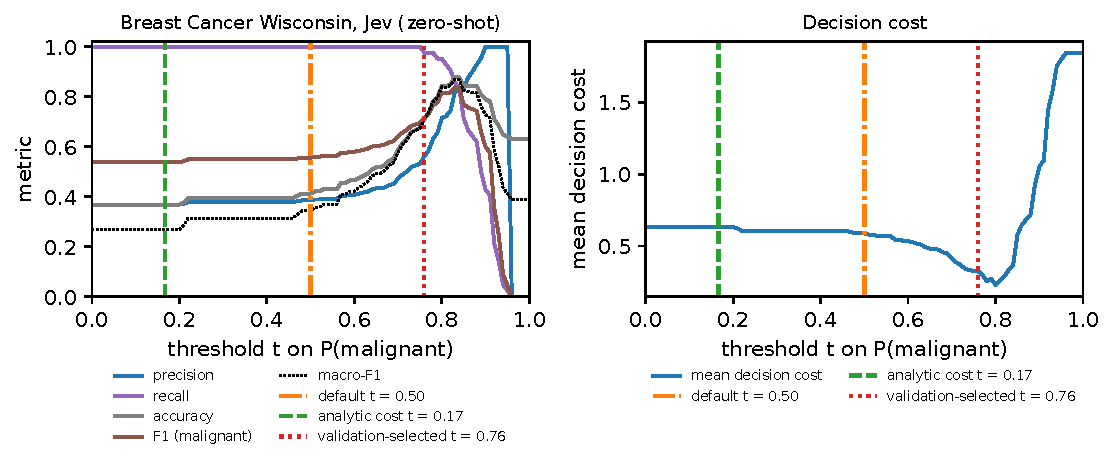
\includegraphics[width=0.86\linewidth]{generated/figs/threshold_wdbc_jev}
  \caption{Jev on Breast Cancer Wisconsin Diagnostic, first split repeat. Left: precision,
    recall, accuracy and positive-class F1 against the threshold $t$ (macro-F1 dashed). Right:
    mean decision cost against $t$. The three thresholds are marked in both panels.}
  \label{fig:threshold}
\end{figure}

Breast Cancer Wisconsin shows what the probabilities are worth when the default decision is not
(Table~\ref{tab:thresholds}, Figure~\ref{fig:threshold}). Jev's probability of \emph{malignant} ranks the rows well but sits
too high. The analytic threshold assumes calibration and moves the wrong way. The
validation-selected threshold moves to $t = \ThresholdValidationJevWdbc$: accuracy rises from
\ThrAccuracyDefaultJevWdbc{} to \ThrAccuracyValidationJevWdbc{} and the cost falls from
\ThrMeanCostDefaultJevWdbc{} to \ThrMeanCostValidationJevWdbc, using \ThrValLabelsJevWdbc{}
labels and no training. It does not close the gap to XGBoost (\ThrMeanCostValidationXgbWdbc).
On German Credit no threshold helps Jev much, because there is little ranking to exploit; for
the calibrated XGBoost the analytic threshold works as theory says, cutting its cost from
\ThrMeanCostDefaultXgbGerman{} to \ThrMeanCostAnalyticXgbGerman. On SST-2, where Jev is already
accurate and calibrated, selection changes little. A model that returns only a label is fixed at
one operating point; a distribution lets about a hundred labels place the decision.
